\subsection{Односторонние производные}
\begin{definition}
    \textit{Односторонние окрестности:}
    $$
    U^{+}_{\delta} (x_{0}) := [x_{0}, x_{0} + \delta) 
    $$
    $$
    U^{-}_{\delta} (x_{0}) := (x_{0} - \delta, x_{0}]
    $$
\end{definition}

\begin{definition}
    Пусть $f:U^{+}_{\delta_{0}} (x_{0}) \mapsto \R.$ Тогда если
    $$\exists \lim\limits_{x \to x_{0} +0} \cfrac{f(x) - f(x_{0})}{x-x_{0}} \in \overline{R},$$

    то он называется \textit{правосторонней производной функции $f$ в точке $x_{0} \ $} и обозначается $f'_{+}(x_{0})$

    Аналогично определяется \textit{левосторонняя производная функции $f$ в точке $x_{0} \ $} и обозначается $f'_{-}(x_{0})$
\end{definition}
\begin{example}
    Рассмотрим $ f(x) = |x|.$

    $$
    f'_{+}(0) = \lim\limits_{x \to +0} \cfrac{|x|}{x} = \lim\limits_{x\to +0} \cfrac{x}{x} = 1;
    $$
    $$
    f'_{-}(0) = \lim\limits_{x \to -0} \cfrac{|x|}{x} = \lim\limits_{x\to -0} \cfrac{-x}{x} = -1.
    $$
\end{example}

\begin{theorem}
    Пусть $f$ дифференцируется в точке $x_{0}$. Тогда $f'_{+}(x_{0}) = f'_{-}(x_{0}) \in \R$. 
\end{theorem}
\begin{proof}
    Функция $f$ дифференцируема в точке $x_{0}$:
    $$
    \exists f'(x_{0}) \in \R \Leftrightarrow \exists \lim\limits_{x \to x_{0} +0}  \cfrac{f(x) - f(x_{0})}{x-x_{0}} = \lim\limits_{x \to x_{0} -0} \cfrac{f(x) - f(x_{0})}{x-x_{0}}.$$
\end{proof}

\subsection{Правила вычисления производных и дифференциалов}
\begin{theorem} \hypertarget{thrm5.3}{}
    Пусть функции $f$ и $g$ дифференцируемые в точке $x_{0}\in \R.$

    Тогда $f \pm g$ и $ f\cdot g$ дифференцируемые в точке $x_{0}$, если $g(x_{0}) \neq 0,$ то $\cfrac{f}{g}$ дифференцируема в точке $x_{0}$

    Более того справедливы равенства: 
    \begin{enumerate}
        \item $(f \pm g)'(x_{0}) = f'(x_{0}) \pm g'({x_{0}}) $
        \item $(f \cdot g)'(x_{0}) = f'(x_{0}) \cdot g({x_{0}}) + f(x_{0}) \cdot g'({x_{0}})$
        \item $\left(\cfrac{f}{g}\right)' (x_{0}) = \cfrac{f'(x_{0}) \cdot g({x_{0}}) - f(x_{0}) \cdot g'({x_{0}})}{g^{2}(x_{0})}, \quad$ $g'(x_{0}) \neq 0$.
    \end{enumerate}
\end{theorem}
\begin{proof}
    Введем обозначения $\Delta f = f (x) - f(x_{0}),\  \Delta g = g(x) - g(x_{0}),\  \Delta x = x - x_{0}$.
    \begin{enumerate}
        \item $\cfrac{\Delta(f \pm g)}{\Delta x} = \cfrac{\Delta f \pm \Delta g}{\Delta x} = \cfrac{\Delta f}{\Delta x} \pm \cfrac{\Delta g}{\Delta x};$
        
        $\cfrac{\Delta f}{\Delta x} \to f'(x_{0}),\  \Delta x \to 0 \quad \quad \cfrac{\Delta g}{\Delta x} \to g'(x_{0}),\  \Delta x \to 0;$

        Тогда $\cfrac{\Delta(f \pm g)}{\Delta x} \to f'(x_{0}) \pm g'(x_{0}), \ x \to x_{0} \Rightarrow (f \pm g)'(x_{0}) \to f'(x_{0}) \pm g'(x_{0}),\  x \to x_{0}.$
        
        \item $\cfrac{\Delta(f\cdot g)}{\Delta x} = \cfrac{f(x) g(x) - f(x_{0}) g(x_{0})}{\Delta x} = \cfrac{f(x) \left[  g(x) - g(x_{0}) \right]}{\Delta x} + \cfrac{g(x_{0}) \left[ f(x) - f(x_{0})\right]}{\Delta x} =$

        $= f(x) \cdot \cfrac{\Delta g}{\Delta x} + g(x_{0}) \cdot \cfrac{\Delta f}{\Delta x}.$

        $\cfrac{\Delta f}{\Delta x} \to f'(x_{0}), \Delta x \to 0 \quad \quad \cfrac{\Delta g}{\Delta x} \to g'(x_{0}), \Delta x \to 0$
        
        $f(x) \to f(x_{0}), \Delta x\to 0,$ так как из дифференцируемости в точке $x_{0}$ следует непрерывность

        Тогда $\cfrac{\Delta (f\cdot x)}{\Delta x} \to f(x_{0}) g'(x_{0}) + g(x_{0})f'(x_{0}),\  \Delta x \to 0 \Rightarrow (f \cdot g)'(x_{0}) = f'(x_{0}) \cdot g({x_{0}}) + f(x_{0}) \cdot g'({x_{0}}).$
        
        \item $\cfrac{\Delta \left(\cfrac{f}{g} \right)}{\Delta x} = \cfrac{\cfrac{f(x)}{g(x)} - \cfrac{f(x_{0})}{g(x_{0})}}{\Delta x} = \cfrac{f(x)g(x_{0}) - f(x_{0})g(x)}{g(x) g(x_{0}) \Delta x}= $

        $=\left(\cfrac{\left[f(x) - f(x_{0})\right] g(x_{0})}{\Delta x} - \cfrac{f(x_{0})\left[g(x) - g(x_{0})\right]}{\Delta x} \right) \cdot \cfrac{1}{g(x) g(x_{0})}, \ g(x_{0}) \neq 0, \  g$ непрерывна в точке $x_{0}.$
        
        Следовательно, переходя к пределу  при $x\to x_{0}$ получим требуемое. 
    \end{enumerate}
\end{proof}

\begin{corollary}
    $ (cf)'(x_{0}) = c\cdot f'(x_{0}) \quad \quad \forall c \in \R
    $
\end{corollary}
\begin{corollary}
    Пусть $f$ и $g$ дифференцируемы в точке $x_{0}$. Тогда выполнено следущее:
    \begin{enumerate}
        \item $  d(f \pm g)(x_{0}) = df(x_{0}) \pm dg({x_{0}}) $
        \item  $ d(f \cdot g)(x_{0}) = df(x_{0}) \cdot g({x_{0}}) + f(x_{0}) \cdot dg({x_{0}})$
        \item $dg(x_{0}) \neq 0 \quad d\left(\cfrac{f}{g}\right) (x_{0}) = \cfrac{df(x_{0}) \cdot g({x_{0}}) - f(x_{0}) \cdot dg({x_{0}})}{g^{2}(x_{0})}$
    \end{enumerate}
\end{corollary}
\begin{theorem}
    \hypertarget{thrm5.10}{(Производная сложной функции)} Пусть $f$ дифференцируема в точке $y_{0}$, $g$ дифференцируем в точке $x_{0}$. Тогда композиция $f \circ g$ дифференцируема в точке $x_{0} $ и $(f\circ g)'(x_{0}) = f'(g(x_{0})) g'(x_{0})$.
\end{theorem}
\begin{note}
     Функция $f$ дифференцируема в точке $y_{0}$, $g$~---~в точке $x_{0}$, значит они определены в некоторой окрестности. Значения функции $g$ попадут в область определения функции $f$, потому что $g$ непрерывна (так как дифференцируема). Значит, для любой окрестности, где определена $f$ найдется такая окрестность, что как только $x$ попадает в нее, то $g(x)$ попадает окрестность, где определена $f$.
\end{note}
\begin{proof}
    Так как $f$ дифференцируема в точке $y_{0},$ то $\exists f'(y_{0}) \in \R$.

    $$f(y) = f(y_{0}) + f'(y_{0})(y-y_{0}) + \epsilon_{1}(y)(y-y_{0}) \quad  \quad   \forall y \in U_{\delta}(y_{0}) \quad \epsilon_{1}(y) \to 0,\quad y\to y_{0};$$
    $$g(x) = g(x_{0}) + g'(x_{0})(x-x_{0}) + \epsilon_{2}(x)(x-x_{0})  \quad \quad  \forall x \in U_{\delta}(x_{0}),\quad \epsilon_{2}(x) \to 0,\quad  x\to x_{0}.$$

    Вместо $y$ подставим $g(x)$
    $$
    f(g(x)) = f(g(x_{0})) + f'(g(x_{0}))\Bigl( g'(x_{0})(x-x_{0}) + \epsilon_{2}(x)(x-x_{0})\Bigr) +  $$
    $$
    + \epsilon_{1}(g(x))\Bigl(g'(x_{0})(x-x_{0}) + \epsilon_{2}(x)(x-x_{0})\Bigr) = (f\circ g)(x_{0}) + f'(g(x_{0}))g(x_{0})(x-x_{0}) + $$
    $$+ \Bigl\{ \epsilon_{2}(x)f'(g(x_{0}))(x-x_{0}) + \epsilon_{1}(g(x))g'(x_{0})(x-x_{0}) + \epsilon_{1}(g(x))\epsilon_{2}(x)(x-x_{0}) \Bigr\}$$

    $$
    \{\} = (x-x_{0})\Bigl[\epsilon_{2}(x)f'(g(x_{0})) + \epsilon_{1}(g(x))g'(x_{0}) + \epsilon_{1}(g(x))\epsilon_{2}(x) \Bigr] = (x - x_{0}) \cdot \epsilon(x) \quad \epsilon(x) \to 0, x\to x_{0}
    $$

    Доопределим $\epsilon_{1}(g(x_{0})) = \epsilon_{1}(y_{0}) = 0$. Тогда $\epsilon_{1}$ становится непрерывной в  $y_{0}.$ И \hyperlink{thrm4.18}{по теореме о замене переменной при вычислении предела} $\epsilon_{1}(g(x))\to 0, x\to x_{0}$
\end{proof}

\begin{theorem}
    \hypertarget{5.11}{(Производная обратной функции)} Пусть $y: U_{\delta}(x_{0}) \mapsto \R$ строго монотонна и непрерывна в этой окрестности. Пусть $y'(x_{0}) \neq 0$. Тогда существует обратная функция $x: U_{\sigma}(y_{0}) \mapsto U_{\delta}(x_{0})$ строго монотонна и непрерывна в $U_{\sigma}(y_{0})$. При этом $x$ дифференцируема в точке $y_{0} = y(x_{0})$ и $x'(y_{0}) = \cfrac{1}{y'(x_{0})}$ 
\end{theorem}
\begin{proof}
    Первая часть теоремы была доказана ранее. Докажем существование производной.

    $$\cfrac{y - y_{0}}{x(y) - x(y_{0})} = \cfrac{1}{\cfrac{x(y) - x(y_{0})}{y(x(y)) - y(x(y_{0}))}} \Leftrightarrow \cfrac{x(y) - x(y_{0})}{y - y_{0}} = \cfrac{1}{\cfrac{y(x(y)) - y(x(y_{0}))}{x(y) - x(y_{0})}}$$
    
    $y(x)$ и $x(y)$ взаимообратны.

    Так как $x(y)$ осуществляет биективное отображение $U_{\delta} (y_{0}) \mapsto U_{\delta}(x_{0})$, то $x(y) \neq x_{0} $ при $y \neq y_{0}$. Из непрерывности $x(y)$ в точке $y_{0}$ следует $\exists \lim\limits_{x \to x_{0}} x(y) = x(y_{0}).$
    Следовательно, можно воспользоваться \hyperlink{thrm4.17}{теоремой о замене переменной при вычислении предела}.
    
    $$\exists \lim\limits_{y\to y_{0}} \cfrac{1}{\cfrac{y(x(y)) - y(x(y_{0}))}{x(y) - x(y_{0})}} = \lim\limits_{x \to x_{0}}  \left( \cfrac{y(x) - y(x_{0})}{x - x_{0}}\right)^{-1} = \cfrac{1}{y'(x_{0})} = x'(y_{0})$$    
\end{proof}
\begin{corollary}$\ $

\begin{table}[h]
\begin{tabular}{llllll}
1. & $a^{x} = a^{x} \cdot \ln a$, $\ \forall a \in (0; +\infty)$, & $x\in \R$ & 8. & $(\ln x)' = \cfrac{1}{x}$, & $x \in \left( 0; +\infty\right)$\\
2. & $(\sin x)' = \cos x$, & $x \in \R$ & 9. & $(\arctan x)' = \cfrac{1}{1 + x^{2}}$, & $x \in \R$\\
3. & $(\cos x)' = - \sin x$, & $x \in \R$ & 10. & $(\arcctg x)' = \cfrac{-1}{1 + x^2}$, & $x \in \R$\\
4. & $(\tg x)' = \cfrac{1}{\cos^{2} x}$, & $x \in \R$ & 11. & $(\sh x)' = \ch x$, & $x\in \R$ \\
5. & $(\ctg x)' = -\cfrac{1}{\sin^{2} x}$, & $x \in \R$ & 12. & $(\ch x)' = \sh x$, & $x\in \R$\\
6. & $(\arcsin x)' = \cfrac{1}{\sqrt{1 - x^{2}}}$, & $x \in \left(-\cfrac{\pi}{2}; \cfrac{\pi}{2}\right)$ & 13. & $(\th x)' = \cfrac{1}{\ch^{2} x}$, & $x\in \R$\\
7. & $(\arccos x)' = -\cfrac{1}{\sqrt{1-x^{2}}}$, & $x \in (0; \pi)$ & 14. & $(\cth x)' = -\cfrac{1}{\sh^{2} x}$, & $x\in \R$\\
\end{tabular}
\end{table}
\end{corollary}
\begin{proof} $\ $
    \begin{enumerate}
        \item  $\cfrac{e^{x} - e^{x_{0}}}{x-x_{0}} = e^{x_{0}}\cfrac{(e^{x-x_{0}}-1)}{x-x_{0}} \to e^{x_{0}}, x\to x_{0}\Rightarrow (e^{x})' = e^{x}$
            
        $(a^{x})' = (e^{\ln a \cdot x})' = e^{y(x)} \cdot y'(x) = a^{x} \cdot \ln a, \quad y(x) = \ln a\cdot x$.
        
        \item $\cfrac{\sin x- \sin x_{0}}{x - x_{0}} = \cfrac{\sin (x_{0} +\Delta x) - \sin x_{0}}{\Delta x} $ \small$=\cfrac{\sin x_{0} \cdot \cos (\Delta x) + \cos x_{0} \cdot \sin (\Delta x) -\sin x_{0}}{\Delta x} $\normalsize$ = \cos x_{0} $.
        
        \item
            Редукция с помощью сдвига на $\cfrac{\pi}{2}$.
        \item
            $(\tg x)' = \left( \cfrac{\sin x}{\cos x} \right)'= \cfrac{\cos x\cdot \cos x + \sin x \cdot \sin x}{\cos^{2} x}  \cfrac{1}{\cos^{2} x}$
        \item
            Аналогично $(\tg x)'$.
        \item
            $(\arcsin x)' = \cfrac{1}{\cos(\arcsin x)} = \cfrac{1}{\sqrt{1-\sin^{2}(\arcsin x)}} = \cfrac{1}{\sqrt{1 - x^{2}}}$.
        \item
            Аналогично $(\arcsin x)'$.
        \item
            $y'(x) = (\ln x)' = \cfrac{1}{e^{y(x)}} = \cfrac{1}{e^{\ln x}} = \cfrac{1}{x}$.
        \item
            $(\arctan x)' = \cfrac{1}{\cfrac{1}{\cos^{2}(\arctan x)}} = \cfrac{1}{1+x^{2}}$.
        \item
            Аналогично $(\arctan x)'$.
        \item
            Задание на дом:)
        \item
            Задание на дом:)
        \item
            $(\th x)' =\left(\cfrac{\sh x}{\ch x}\right)' = \cfrac{\ch x \cdot \ch x - \sh x \cdot \sh x}{\ch^{2} x} = \cfrac{1}{\ch^{2} x} $.
        \item
            $(\th x)' =\left(\cfrac{\ch x}{\sh x}\right)' = \cfrac{\sh x \cdot \sh x - \ch x \cdot \ch x}{\sh^{2} x} = \cfrac{-1}{\sh^{2} x} $.
    \end{enumerate}
\end{proof}

\subsection{Производные и дифференциалы высших порядков}
\begin{definition}
    $f^{0} = f(x), f'(x)$ определили. ($f'(x)$~---~ функция точки $x$).

    Далее по индукции. Если в некоторой окрестности точки $x_{0}$ определена $f^{(n)}(x)$, то $f^{(n+1)} (x_{0}) = \left(f^{(n)}\right)'(x_{0})$
\end{definition}

\begin{definition}
    Пусть $f$ дифференцируема в окрестности точки $x_{0}$ и $\exists f''(x_{0})$. Тогда \textit{дифференциалом 2-ого порядка функции f в точке $x_{0}$} называется дифференциал от дифференциала 1-ого порядка как функции точки $x$ при фиксированном $dx$
\end{definition}

\sidefig(10 cm)(7 cm)
{
\begin{flushleft}
\normalsize
То есть $d^2 f(x) := d\Bigl(df(x)\Bigr)$

В каждой точке графика построим касательную. Взять дифференциал от дифференциала означает следущее. $df(x)$~---~ семейство этих касательных. У каждой касательной нужно зафиксировать приращение (на рисунке отмечено жирными точками). Таким образом наша функция - огибающая этих приращений. Ее и нужно дифференцировать.
\end{flushleft}
}
{
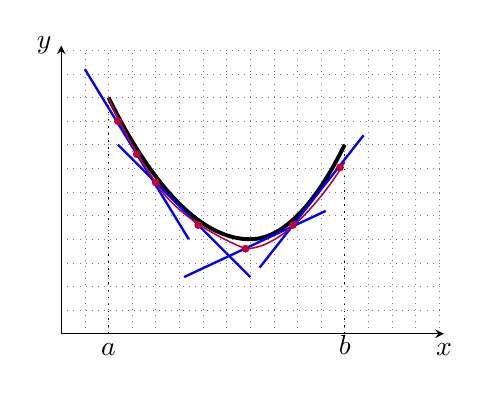
\begin{tikzpicture}[>=stealth, scale =1.2]
		% Рисуем сетку
		\draw[help lines, step=0.25, dotted]
		(0,0) grid (4,3);
		% Начало координат
		\draw[->, thin] (0,0) -- (4.05,0)
		node[below] {$x$}; % Ox
		\draw[->, thin] (0,0) -- (0, 3.05)
		node[left] {$y$}; % Oy
		
		\draw[line width =.02cm, dotted] (0.5, 0) -- (0.5, 2.5);
		\draw[line width =.02cm, dotted] (3, 0) -- (3, 2);
		
		\draw[line width =.05cm](0.5, 2.5) parabola bend (2, 1)(3, 2);
		
		\draw[line width =.03cm, blue] (0.25, 2.8) -- (1.35, 1);
		\draw[line width =.03cm, blue] (0.6, 2) -- (2, 0.6);
		\draw[line width =.03cm, blue] (1.3, 0.6) -- (2.8, 1.3);
		\draw[line width =.03cm, blue] (2.1, 0.7) -- (3.2, 2.1);	
		
		\draw [fill = purple,purple] (0.6,2.25) circle (1pt);
		\draw [fill = purple,purple] (0.8,1.9) circle (1pt);
		\draw [fill = purple,purple] (1,1.6) circle (1pt);
		\draw [fill = purple,purple] (1.45,1.15) circle (1pt);
		\draw [fill = purple,purple] (1.95,0.9) circle (1pt);
		\draw [fill = purple,purple] (2.45,1.15) circle (1pt);	
		\draw [fill = purple,purple] (2.95,1.76) circle (1pt);
								
		\draw[line width =.02cm, purple] (0.5, 2.5).. controls (0.6,2.25) and (0.8,1.9) .. (1,1.6);
		\draw[line width =.02cm, purple] (1,1.6) .. controls (1.28,1.15) and (1.95,0.9) .. (1.95,0.9);
		\draw[line width =.02cm, purple] (1.95,0.9) .. controls (2.45,0.9) and (3,1.8) .. (3,1.82);
		
		\node[below] at (0.5, 0) {$a$};
		\node[below] at (3, 0.085) {$b$};
		
		
\end{tikzpicture}

}


    

\begin{definition}
    Если определён $d^{(n)}f(x)$ в некоторой окрестности точки $x_{0}$ и $\exists f^{(n+1)}(x_{0})$, то $d^{(n+1)} f(x_{0}) :=  d\Bigl(d^{(n)}f(x)\Bigr)(x_{0})$
\end{definition}

\begin{theorem}
    Пусть $n\in N, \ \exists f^{(n)}(x_{0})$. Тогда  $d^{(n+1)} f(x_{0}) = f^{(n)}(x_{0}) (dx)^{n}$ 
\end{theorem}
\begin{proof}
    Докажем по индукции. При $n = 1$ очевидно.

    При $n \geq 2$ пусть $\exists f^{(n)}(x_{0})$.

    $$
    d^{2} f(x_{0}) = d\Bigl(df(x)\Bigr) \Bigr|_{x = x_{0}} = d\Bigl(f'(x)dx\Bigr)(x_{0}) = f''(x_{0})(dx)^{2}
    $$

    Пусть формула доказана при $k \in \N$

    $$
    1 \leq k\leq n-1 \quad d^{k} f(x_{0}) = d\Bigl(d^{k} f(x)\Bigr)(x_{0}) = d\Bigl(f^{(k)}(x_{0}) (dx)^{k}\Bigr) = f^{(k +1)}(x_{0})(dx)^{k+1}
    $$
    
\end{proof}